\documentclass{article}
\usepackage[utf8]{inputenc}

\title{DECO-X - Developer Collaboration Explorer}
\author{Ming-Hung Lu \\ Department of Computer Science, University of California, Davis \\ miclu@ucdavis.edu}
\date{}
\usepackage{natbib}
\usepackage{graphicx}

\begin{document}


\begin{titlepage}
    \begin{center}
        \vspace*{1cm}
        \textbf{DECO-X - Developer Collaboration Explorer}
    
        \vspace{0.5cm}
        
        By
        
        \vspace{0.5cm}

        \textbf{Ming-Hung Lu \\ miclu@ucdavis.edu}
        
        \vspace{0.5cm}
        
        A PROJECT REPORT
        
        \vspace{0.5cm}
        
        Submitted in partial satisfaction for the requirements of the degree of
        
        \vspace{0.5cm}
        
        
        MSATER OF SCIENCE
        
        \vspace{0.5cm}
        in
        \vspace{0.5cm}
        
        Computer Science

        \vspace{0.5cm}
        
        in the
        
        \vspace{0.5cm}
        
        OFFICE OF GRADUATE STUDIES
        
        \vspace{0.5cm}
        
        of the
        
        \vspace{0.5cm}
        
        UNIVERSITY OF CALIFORNIA
        
        \vspace{0.5cm}
        
        DAVIS
        
        \vspace{0.5cm}
        
        \textbf{Advising Professors: \\ Vladimir Filkov, Ph.D \\ Premkumar Devanbu, Ph.D }
        
        \vfill
        
        \vspace{0.8cm}
        
        2017
        
    \end{center}
\end{titlepage}


% \maketitle

\section{Introduction}
In large open source software projects, many developers collaborate together to develop and maintain the project. There are almost countless factors that will affect such collaborations. Factors such as: developers' backgrounds, preferred programming language, preferred working time, interests etc. all likely to play a role in determining who each developer collaborates with. Study of such collaboration is particularly interesting in online open source projects, where potentially developers across the globe from different countries, ethnic background and training all working together.
\subsection{Motivation}
From past works, investigating the collaboration between developers is of high interest. In the following, we discuss several sample scenarios in ``COOSOFT," a fictional OSS project, to show that discovering collaboration can greatly assist the development of a project and how our tool can help in each of the cases\\
\begin{itemize}
    \item \textbf{Scenario 1:} Vlad is a new developer coming on board, he might want to discover what's the ``popular" feature that everyone was working on in the past couple weeks to get him familiarized with the project. Our proposed tool can help Vlad discover what is the popular feature being worked on in any time frame he chose. This is discussed in more detail in 3.2.
    \item \textbf{Scenario 2:} Prem, a developer working exclusively on device driver related features, might want to find out who in this project is focused on, say, operating system related features, in order to assist him in developing compatible drivers for the system. Because of the intuitive visualization interface, our tool will be able to help Prem quickly find the principle developers of operating system related feature. This is discussed in more detail in 3.4. 
    \item \textbf{Scenario 3:} Cindy, a core developer of COOSOFT, might want to find the dominant developer, if one exists, to promote to the core development team and help her better facilitate the overall development process. Because our tool also provide the user with raw data used for visualization, Cindy can utilize our tool to quickly find who worked on the most files even though our tool did not provide a ``direct" functionality to do so. 
\end{itemize}
From these cases, we can see that if there is a convenient and intuitive visualization tool to help these three developers investigate the collaboration between developers in COOSOFT, they would be able to solve their problems in no time.\\
On the other hand, researchers wishing to quickly test theories and hypothesis of collaboration in OSS projects can also utilize such tool to effortlessly investigate several OSS projects. For example, Casey, a researcher in an university, might want to investigate the feature focuses of the majority of the developers in COOSOFT at a particular time. Without an interactive tool, he would have to sift through large amount of commit records in order to discover such focus. With our tool, he can effortlessly test several features and discover which one is the focus on the majority of the developers.\\
\subsection{Related Works}
In the past, there has been several studies on the collaboration of developers in online open source software (OSS) projects. In the following discussed works, the authors all found some interesting phenomenon in OSS project collaboration. In a paper by Posnett et al.\citep{posnett2013dual}, the authors found that OSS projects' developers tend to have different working styles because of the lack of formal assignment of tasks by, say, a software company's management. Some developers might focus on specific features while others might switch between different features. This suggests that the collaboration in OSS projects could be quite different than say, a company managed software project, since the working style of each developer could differ quite drastically. Also, it might mean that it is harder to collaborate in OSS projects since people with different habits cannot easily work well together. The author also discovered that there are ``dominant" contributors in OSS projects, meaning some developers put in significant more work than others. If it were true, then discovering such ``dominant developers" might be very helpful for the continued development of the project. In a more recent work by Xuan et al.\citep{xuan2014focus}, the authors found that in several OSS projects, developers' focus tend to shift over time . The authors further correlated such shifting of focuses with the project's file dependencies via analysis of the call graph. Several interesting question came out of such finding. First, if developers' focuses shift over time, then at a particular time period, what are the developers' focuses? Second, do all developers' focuses shift at the same time and rate? Or maybe some shift focus while others still focus on the old feature. In anther work by Xuan et al.\citep{xuan2016converging}, the authors found that the ``work-talk" pattern of developers in a OSS project tend to converge over time . In this paper, the ``work-talk" pattern is the pattern of a particular developer's habit of switching between ``working," i.e. writing codes and committing to repositories, and ``talking," i.e. discussing with other developers through e-mail communications. Over time, the pattern of the majority of the developers in a particular OSS project tend to converge, implying a form of collaboration emerging. The authors also found that developer tend to stay in the same kind of activity instead of switching constantly between them \citep{xuan2016converging}. In another more recent work by Vasilescu et al.\citep{vasilescu2016sky}, the authors investigated several Github projects and found that multitasking might improve productivity. However, extensive multitasking actually decreases productivity. This also raises interesting questions. If multitasking excessively decreases productivity, then can we discover if a developer is multitasking excessively?\\
On the other hand, several visualization tool exists to help with investigating software collaborations. In a previous work by Hattori et al.\citep{hattori2010syde}, the authors proposed a tool ``Syde" that help the development team collaborate better by sharing critical software information. Syde seemed very effective in conveying code related information such as ``effort spent on each class"\citep{hattori2010syde} with an intuitive ``bucket" graph. This can potentially be very useful in discovering what's the feature focus of the entire repository. However, the tool doesn't seemed to be very helpful in visualizing the collaboration between developers and their activities throughout time. In another work by de Souza et al.\citep{de2007supporting}, the authors proposed a tool, Ariadne, that can visualize the dependencies along with authorship information. In their paper, the discussed scenario 3 and 4 is particularly interesting. In scenario 3, the author presented Ariadne's ability to visualize the developers responsible of dependencies which is very useful in identifying who is the right person to talk to about a particular feature\citep{de2007supporting}. In scenario 4, the authors showcased Ariadne's ability to find developer working on the same features which is also very helpful for a developer trying to find peers to collaborate with. However, it appears Ariadne also did not have a way to visualize the ``change over time" in both cases. As we discovered from prior works by Xuan et al.\citep{xuan2014focus}, developers' focuses shift over time in OSS projects. As such, a developer who built a particular feature might not be the developer who is currently maintaining the feature and they might be able to provide more help than the original developers. On the other hand, our proposed tool attempt to address such limitation by providing an interactive Sankey diagram which helps with visualizing ``history," this is discussed in more detail in 2.6.
\section{DECO-X}
We propose a novel tool, DECO-X (DEveloper COllaboration eXplorer), to automatically discover and visualize collaboration in OSS projects. In specific, DECO-X's backend processing is made in Python programming language and works with OSS projects on Github, an online hosting service for many popular projects. DECO-X focuses on the activity of developers throughout the history of a Github project and how they interact with each other. As such, developers involved in the project can use it to discover phenomenons in the project and researchers can use it to test hypothesis and theories regarding collaboration in Github projects. Unlike pure statistical analysis, DECO-X offers an interactive web-based interface allowing the user to examine long collaboration history with ease. DECO-X is an end-to-end pipeline that processes records of a Github project, performs analysis and produces results which can be visualized by the included user interface (UI). In the pipeline, several modular components reads data from previous stage and produces data to feed into the next stage. This allows easy modification of methodologies or libraries without affecting the overall functionality. Figure \ref{fig:pipeline} illustrates each component of the pipeline and their relationship to other components. The details of each stage of the pipeline as well as some potential modifications is discussed in following sections. DECO-X utilizes PyGithub\footnote{PyGithub can be found under https://github.com/PyGithub/PyGithub} to connect to Github and gather data directly so it does not depend on any pre-compiled database such as GHTorrent\citep{Gousi13}, although existing data could potentially help speed up the processing time. DECO-X also has the ability to keep track of developers across different Github projects it is possible to analyze several projects together.
\begin{figure}[h!]
\centering
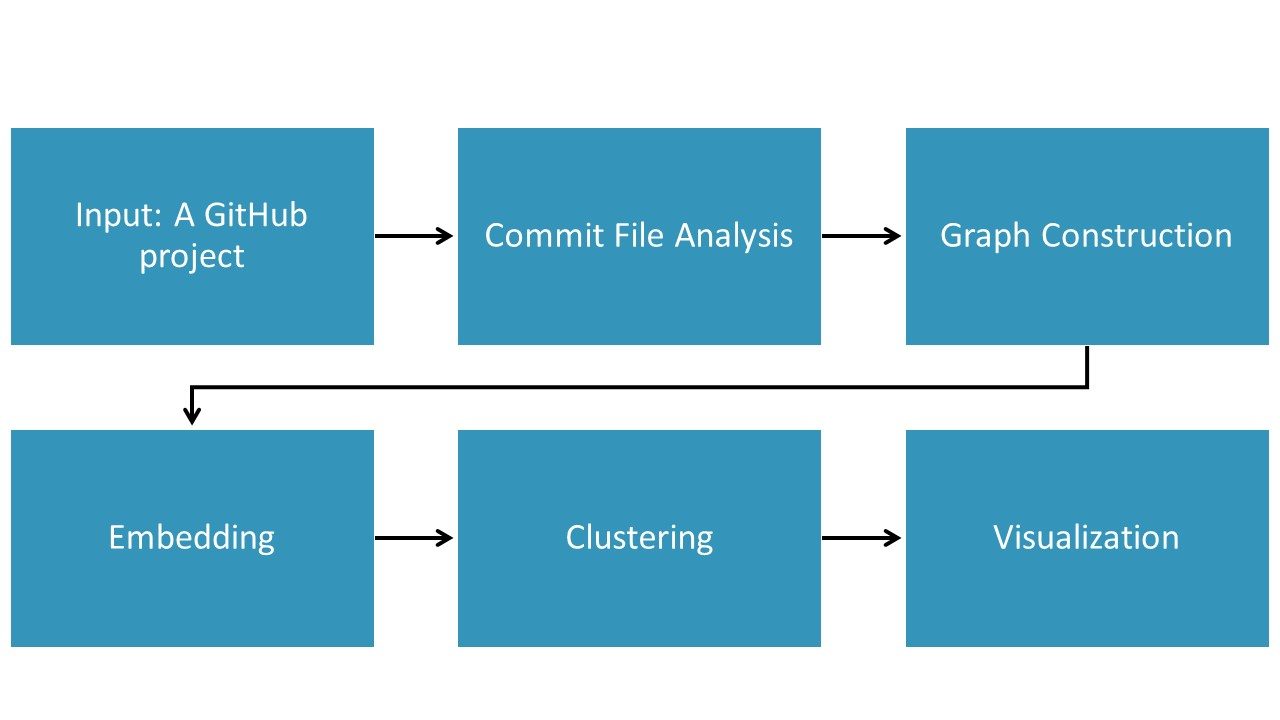
\includegraphics[scale=0.3]{images/pipeline.jpg}
\caption{DECO-X Pipeline}
\label{fig:pipeline}
\end{figure}

\subsection{Input}
As shown in Figure \ref{fig:pipeline}, the input to DECO-X is any Github project. Each project is identified by the project's owner username and the repository name. For example, a repository named ``coosoft" under user vlad123 would be given to DECO-X as ``vlad123:coosoft". This is done to separate different fork of the same repository by the different users. The same user could fork a repository under a different name but our tool did not take that into account. DECO-X then get the commits from Github. The final data produced by this stage is a list of commits, sorted in chronological order and a ``developer mapping" that maps a particular developer to an unique number ID. An existing ``developer mapping" is an optional input at this stage to allow DECO-X to process data across projects and might help with processing time.\\
In this report, we picked the project ``ceph:ceph"\footnote{https://github.com/ceph/ceph} (CEPH) to investigate in detail and test our tool. CEPH is a popular distributed object storage system\footnote{http://ceph.com/}. CEPH has a long development history with hundreds of developers and tens of thousands of frequent commits spanning from 2001 until present. We chose CEPH to prevent sparsity of data for the embedding stage. CEPH is also nicely structured so that sub-features of a particular feature is grouped under the same folder (e.g. folder ``src/os" contains codes for operating system related features and ``src" folder, as suggested by the name, contains all the main source code of CEPH), this is important for our graph construction process in 2.3 and visualization in 2.6. Moreover, CEPH has several active developers throughout this period as such it is ideal for collaboration investigations. We have discovered several project that has a high number of developers and commit counts but there are extensive occurrences in which each a developer works individually in separate, long time frames, making it hard to investigate the collobration between them. This is discussed in more detail in 2.3.

\subsection{Commit File Analysis}
Since the commit we gather in stage 2.1 did not have the actual file information. In the second stage, DECO-X parses the list of commits gathered previously and for each commit, it contacts Github for the files committed in that commit. The end data produced by this module is a list of files committed by each developer along with time, as illustrated in Figure \ref{fig:data22}, and a ``file mapping" that maps a particular file to an unique number ID. During the data gathering of CEPH, our tool reported several commits not found and was unable to get file data of those commits. This could happen due to the fact that those commits are deleted from Github. In specific, this happens more frequently for earlier commits than later, more recent ones which might suggest a left censoring condition in our data. Because of this, our subsequent investigation of CEPH focuses on more recent data. Also, since our tool need to connect to Github for the file data of each commit, the processing time for this stage is quite long and we might run into API rate limit. In such a event, our tool provides 2 options for the user. It can automatically sleeps until the limit time is up and resumes processing or stop and return the commit files gathered up to that point. If a pre-compiled list of commit time, developers and files is available, it can substitute the output at this stage and eliminate the need to connect to Github for each commit.

\begin{figure}[h!]
\centering
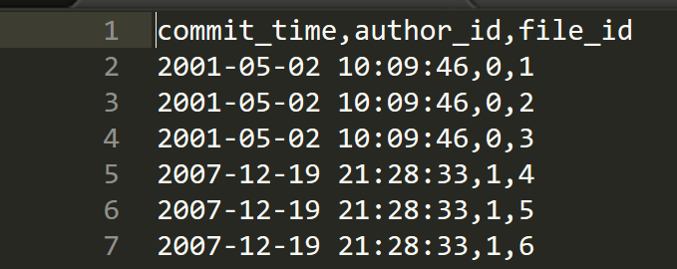
\includegraphics[scale=0.5]{images/datasample.png}
\caption{Sample CSV data produced by 2.2. The first line indicates the header of each column}
\label{fig:data22}
\end{figure}


\subsection{Graph Construction}
In this stage, the user would specify a time frame (e.g. 7 days) he or she wishes to investigate collaboration in. DECO-X reads the file from 2.2 and produces one ``time frame graph" for each of the predetermined time frame over the entire available data. For example, suppose we have commit file data from 5/1/2015 to 6/1/2015 and we want to investigate how each developer collaborated within a week. We would specify 7 days for the time frame and our tool will produce roughly 4 graphs at this stage. In each graph, the nodes are developers who committed a commit in this time frame and each edge between developers mark them as ``related." Several important points to discuss here:\\
First, our tool ignores developer nodes without any edges i.e. dangling nodes. This is mainly because some embedding algorithm used in the next stage did not respond well to dangling nodes in the graph.\\
Second, the meaning of ``related" is a user defined set of criteria that deemed 2 developers related. Some example criteria can be:
\begin{itemize}
    \item 2 developers are related if they touched at least one common file in this period.
    \item 2 developers are related if they touched any file under the same common directory in this period. The level of directory, i.e. how deep this common directory is, can also be a user adjusted.
    \item 2 developers are related if their file touched sequence has a Jaccard index greater than some threshold.
\end{itemize}
Regardless of which criteria used, the purpose here is clear: based on different use cases, the user can define different criteria and ``plug in" this module to produce different graphs for further analysis. In our experiments, we frequently use the first 2 criteria as they directly correlates to features in the CEPH software. Specifically, the second criteria further allows us to tune how deep the level of common directory is. For example, developer A touched file ``src/os/drivers/test.c" and developer B touched file ``src/mon/test/test1.c". A setting of depth of 1 would mean these 2 developers are related as they all touched file under src directory. On the other hand, a depth setting of 2 would mean these 2 developers are not related.\\
Third, the choice of different period might have significant effect on the result. If a particular OSS project's commits aren't frequent, then choosing shorter time frame might cause the graph to have too little data. Conversely, choosing a time frame that is too long might produce an extreme dense graph and fail to capture the collaborations between developers

\subsection{Embedding}
In our pipeline, we included an embedding stage to process the graph and compute ``embedding" for each nodes in each graph. At the end of this stage, the tool will produced one embedding file for each graph containing the embeddings of each node in the respective graph, the embeddings would be later used for clustering. An embedding discussed here is a vector in some high dimensional space that represent a node in the graph. This is very similar to the idea of ``word embedding" used in natural language processing (NLP) where each word in an article is embedded by a high dimensional feature vector. Based on different use cases, the user might want to adjust the embedding techniques to discover different types of ``community." For example, the user may want to discover communities based on which features, in a particular OSS project, a group of developers frequently worked on. As such, this can translate to nodes closer to each other in the graph constructed using the method mentioned in 2.3. On the other hand, the user may define ``community" as a set of developer who serves similar function in a OSS project. So the user might want developers that frequently touch a lot of different features be grouped together and developers that only work locally on a particular feature for extended period of time be grouped separately. This would translate to finding nodes that are structurally equivalent in a graph constructed before. Several embedding techniques can be used in this module such as Node2Vec\citep{grover2016node2vec} and DeepWalk\citep{perozzi2014deepwalk}.\\
To accommodate for different use cases, we decided to incorporate Node2Vec as our embedding technique. We chose Node2Vec because it allows the user to adjust 2 parameters, $P$ and $Q$, to tune the algorithm to embed nodes with different meanings. Also, Node2Vec is avaliable in Python and highly scalable. According to Grover et al.\citep{grover2016node2vec}, setting $P = 1$ and $Q = 0.5$ would correspond to discovering local communities, i.e. nodes that are ``closer" in the graph would be embedded closer. On the other hand, setting $P = 1$ and $Q = 2$ would correspond to embedding structural equivalent nodes closer\citep{grover2016node2vec}. In our experiments, we primarily used a setting of $P = 1$ and $Q = 0.5$ to embed developers who likely worked on similar features closer. 

\subsection{Clustering}
After embedding of each graph is calculated, the clustering stage would take these data and output one cluster file for each graph. Each of the cluster file contains what cluster does each node belongs to. Figure \ref{fig:clustering} is a visualization of a single cluster file, generated using R, with the corresponding graph file constructed in 2.3. The color of each node indicates which cluster it belongs to and the size of each node represent the degree of the node. In this graph, the embedding parameters used are $P = 1$ and $Q = 0.5$ and we can observe several clusters being formed. In specific, we can see that the orange cluster is a small, compact cluster. This highly suggests that this group of developers are working on some features that others did not work on, as indicated by the fact that the orange developer nodes has little to no edge connecting to non-orange developer nodes.
\begin{figure}[h!]
\centering
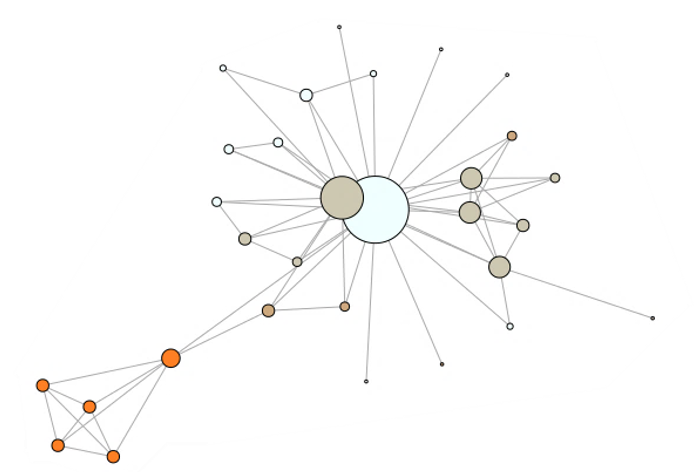
\includegraphics[scale=0.5]{images/cluster.png}
\caption{Visualization of a sample cluster using data from 2.3, 2.4 and 2.5}
\label{fig:clustering}
\end{figure}
Because of the modular design, different clustering algorithm can be substituted in this stage. We mainly focus our experiments on 2 different types of clustering algorithms: hierarchical clustering and k-means clustering. In the following, we discuss the pros and cons of each type:\\
First, we attempted hierarchical clustering (HC). The major benefit of HC is that it does not require ``number of clusters" as an input. To actually get the clusters, we would cut the HC tree at some height to obtain the actual clusters. The algorithm automatically group nodes together and number of cluster is dynamic from graph to graph. On the other hand, the decision of which height to cut the HC tree at is a challenging one. If the algorithm were to cut at a fixed height, say, 0.4, there is no guarantee that 0.4 can accurately portray the clusters in all graphs. During our experiments, we found that cutting the HC tree at a fix height often caused many graphs to have all nodes in one cluster. To remediate such issues, we tried using some statistical methods to dynamically cut at different height for different graphs. For example, cutting each HC tree at 90 percentile height guarantees that there are at least 2 clusters. However, it is then difficult to justify such decision. I.e. why make a choice of 90 percentile instead of, say, 80 percentile?\\
To overcome such issue, we developed another approach with k-means clustering (KM). With KM, the first challenge is that the number of cluster is required as an input to the clustering algorithm, which means we would have to know the number of cluster in each graph in the first place. To come up with the correct number of cluster is a difficult task as it is almost for certain that the collaboration between developers changes from time to time. For example, there might be a lot of small clusters in one time period where each of the groups are focusing on a feature while a few big clusters in another time period where the developers are integrating features together. In an attempt to tackle such problem, we first theorize that at each time frame, the number of cluster is $f(n)$ where $n$ is the number of developers present in the current time frame. Moreover, we used some sub-linear functions such as $\sqrt{n}$ or $\log{n}$ to represent the number of clusters. This is based on the fact that first, if there are more developers in a graph, it is more likely that they are working on more different features. Second, it is unlikely that the number of clusters grows linearly with number of developers since there isn't that many feature to focus on. Based on the results from Vasilescu et al.\citep{vasilescu2016sky}, multitasking too extensively damages productivity and we think that developers in CEPH did not multitask too much since their productivity are quite high based on commit records. We discovered that using KM clustering with a theorized number of clusters appears to produced better results. At the very least, KM clustering overcame the cases where HC produces one single cluster for all nodes.\\
Also, our tool can have the options to partition the whole set of graphs into several parts in order to not overwhelm the visualization interface. For example, if the entire project analyzed has 300 graphs, the user can choose to partition them into 60-graphs chunk and the tool will automatically output 5 chunks.

\subsection{Visualization and Interface}
After all the processings are done, the data are compiled in separate files and DECO-X's web based interface can load the files and produce an interactive graph for the user to explore the developer collaborations. The interface uses D3.js\footnote{Can be found at https://d3js.org/}, a free popular JavaScript based visualization library used in industries. Figure \ref{fig:interface} shows the user interface of DECO-X. At the top is the main menu that allows the user the interact with the Sankey diagram, which is populated in the middle section. The bottom 3 columns shows supportive information about a developer or a cluster selected by the user. The following explains each sections in detail.\\
\begin{figure}[h!]
\centering
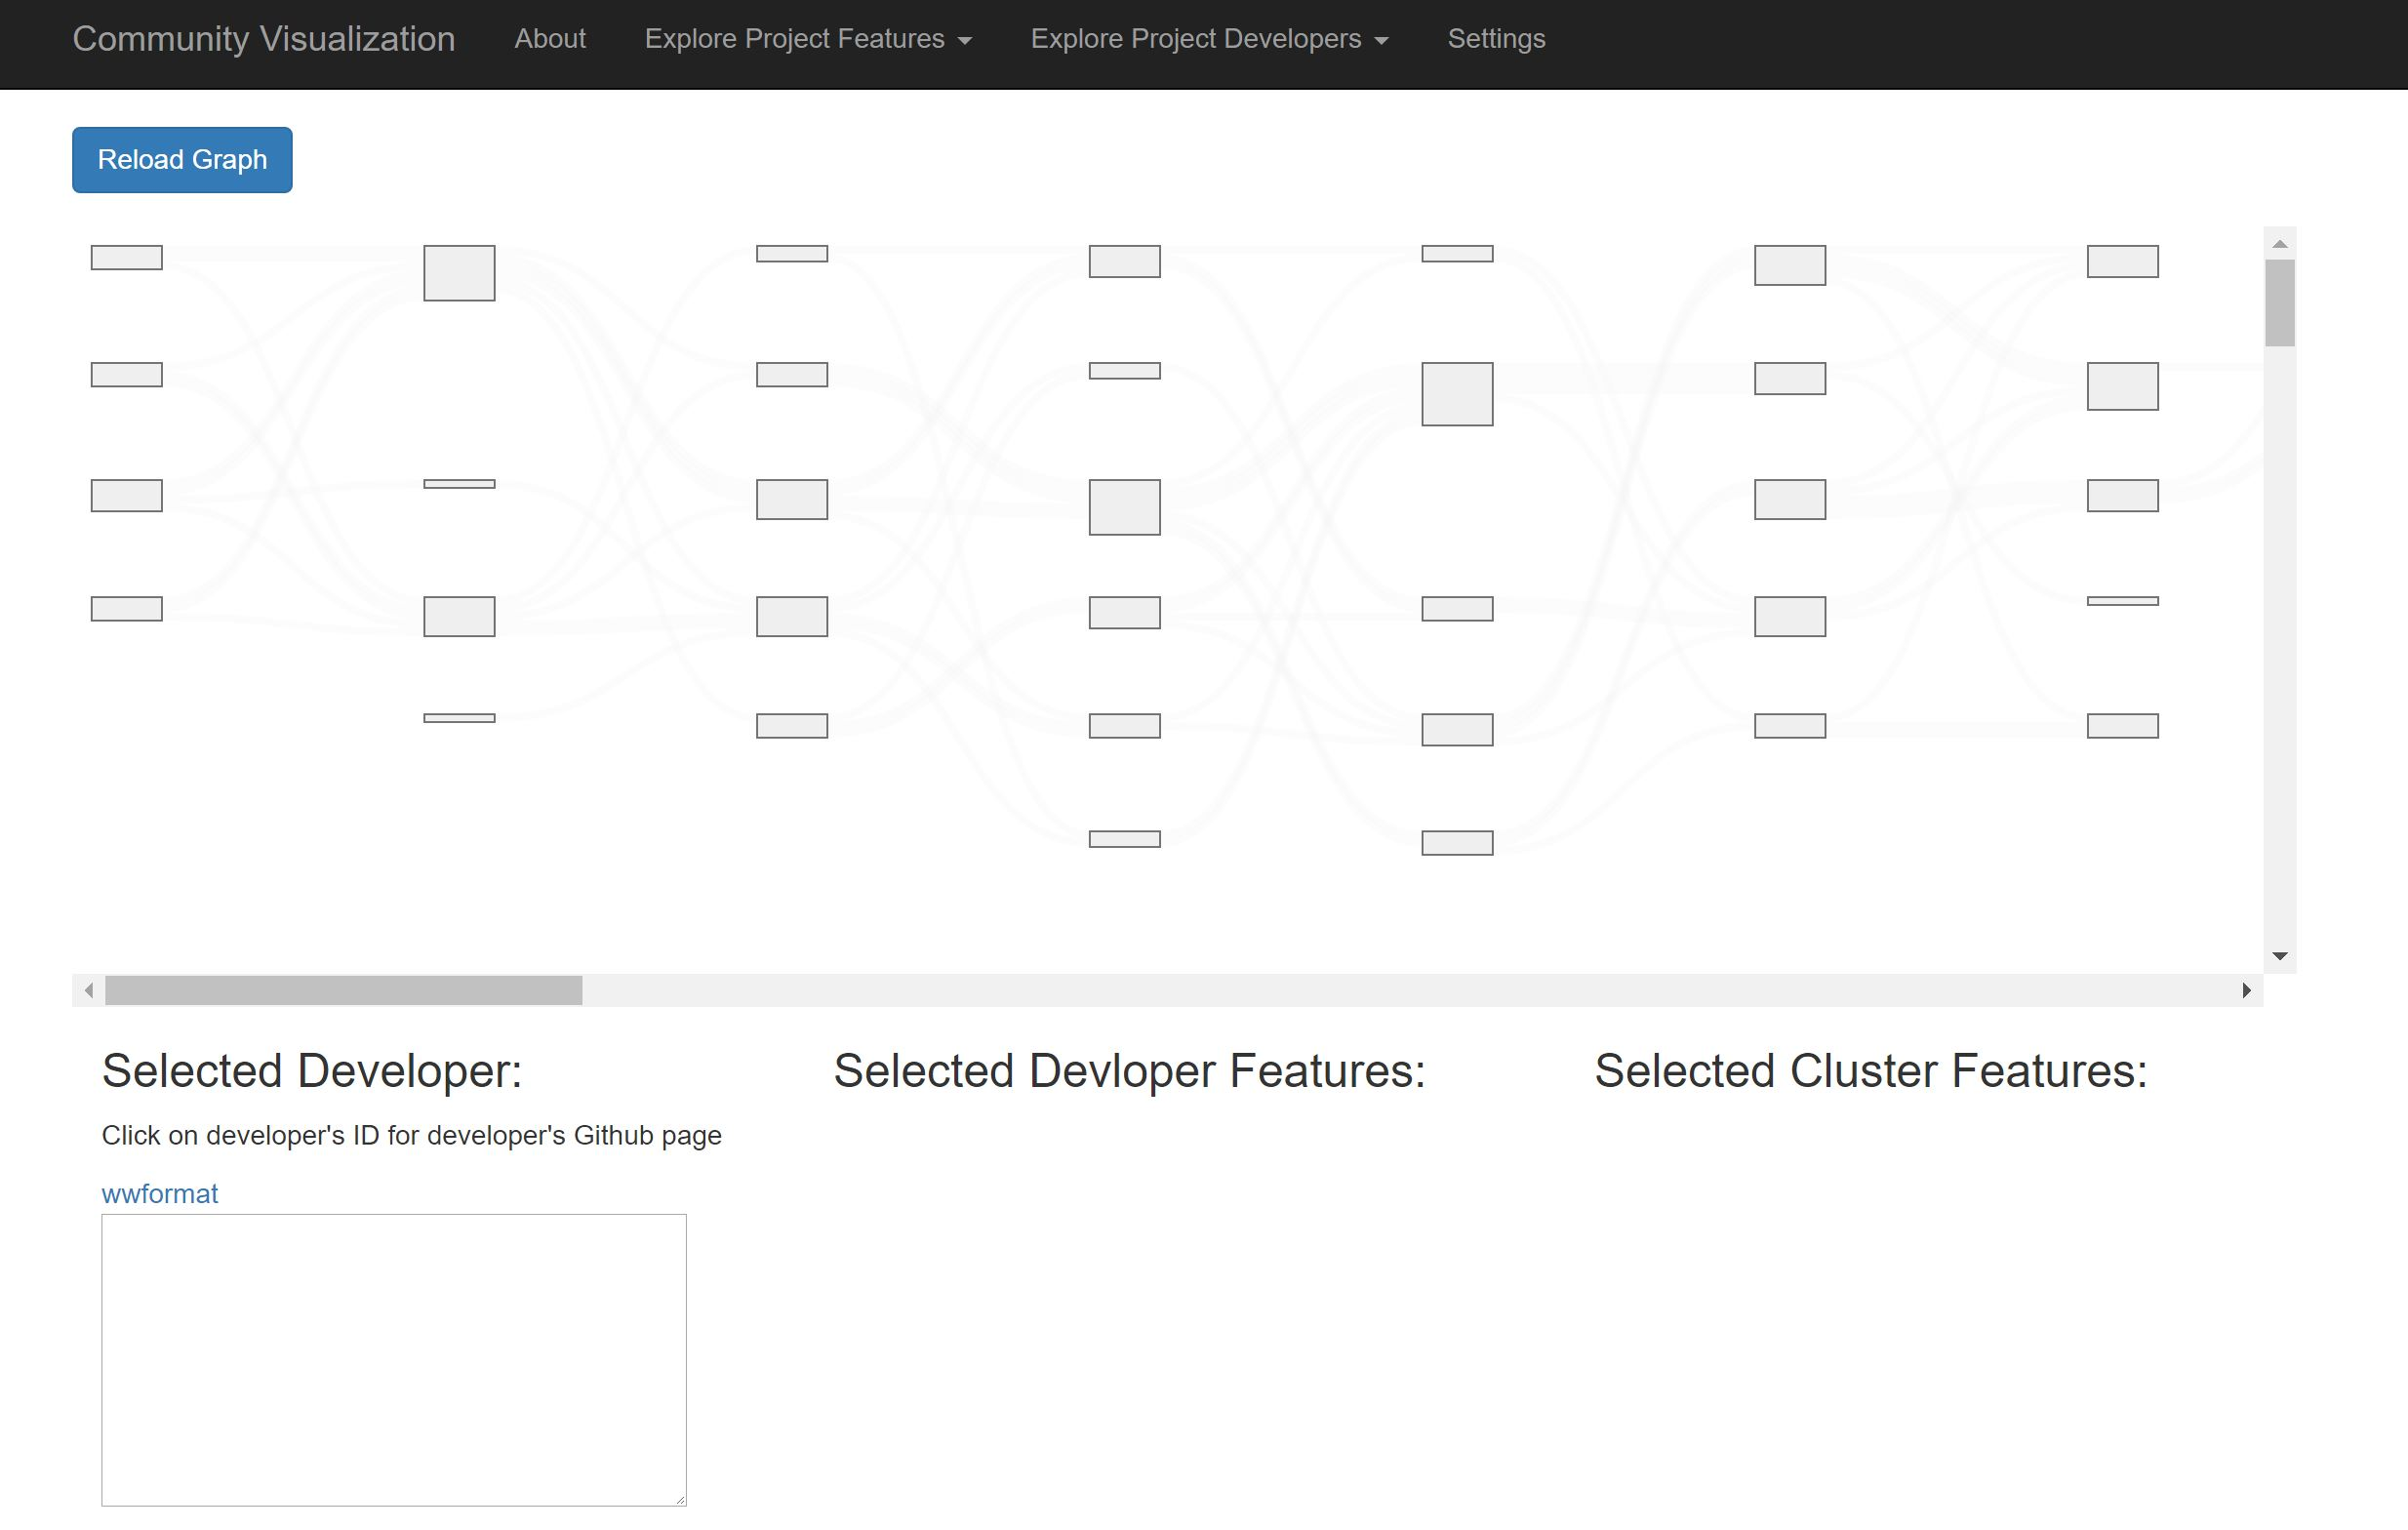
\includegraphics[scale=0.4]{images/interface.JPG}
\caption{Web interface of DECO-X}
\label{fig:interface}
\end{figure}
At the center of the interface is the visualization graph generated based on data produced before. In order to visualize the clusters of developers as well as how each developer moves between clusters, we choose to use a Sankey diagram\footnote{D3 Sankey diagram code derived from Mike Bostock's example https://bost.ocks.org/mike/sankey/ and D3 Sankey plugin https://github.com/d3/d3-plugins/tree/master/sankey} to visualize the data. Sankey diagrams are used in many studies to visualize ``flows." According to Schmidt et al.\citep{schmidt2008sankey}, Sankey diagram has been used in the study of heat transfer and energy flows dating back to mid to late 90's. In our application, we use Sankey diagram to visualize the flow of developers moving from one cluster to another between time frames. At the start of the tool, the user would be prompted to enter the file name of the Sankey diagram he or she wishes to investigate. Figure \ref{fig:sankeysample} shows a section of a sample Sankey diagram produced by DECO-X.\\
\begin{figure}[h!]
\centering
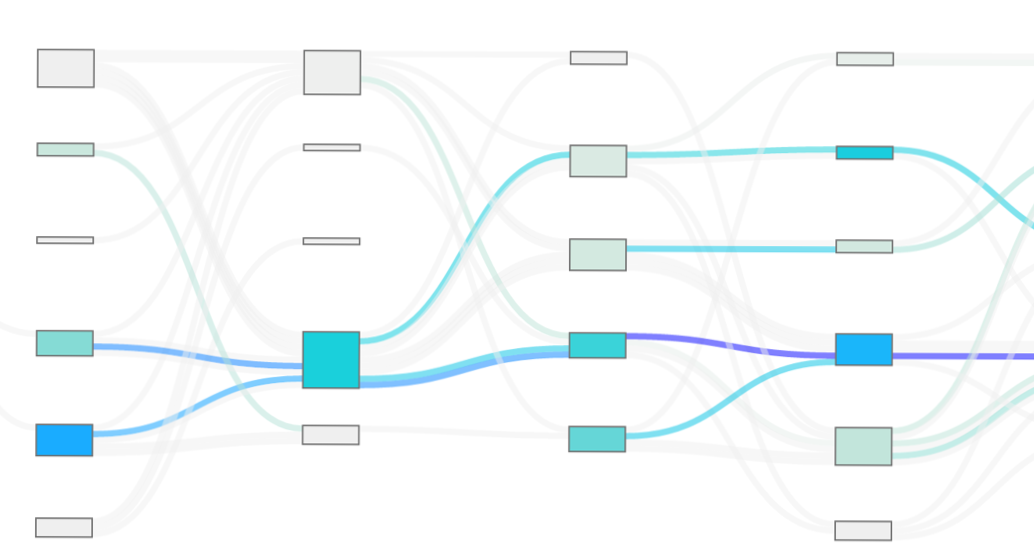
\includegraphics[scale=0.4]{images/sankeySample.png}
\caption{A Sankey diagram produced by DECO-X, colors are added for display purposes}
\label{fig:sankeysample}
\end{figure}
First, each time frame graph is represented by a vertical set of boxes in Figure \ref{fig:sankeysample}, each line connecting 2 boxes between vertical sets of boxes represents a developer moving from one cluster to another. The colors, in this case, are added for demonstration purposes. Under different use cases, our tool automatically add in colors to assist in the investigation of developers' flows and collaborations, this is discussed in more details in section 3. There are several benefits of using a Sankey diagram. First, as each box's size is proportional to the number of developers, we can easily see how each cluster of developers compare to others in terms of sizes. Second, with the lines connecting boxes together, we can easily identify which developers stays together or split up from one time frame to another.\\
The main menu assists user in manipulating the Sankey diagram which is built upon the popular Bootstrap framework\footnote{www.getbootstrap.com}. The main functions are divided into use cases which are group into 2 categories: project feature exploration and project developer exploration. Developer exploration contains use cases about developers such as searching a developer by his or her Github username. On the other hand, feature exploration contains use cases focusing on the project's features such as highlighting which developer touched a given feature. In DECO-X, a ``feature" is a particular folder in the project, as discussed before in 2.1.\\
The bottom 3 columns displays more information about a particular developer or cluster selected by the user. To select a developer, the user only need to click on one of the lines and DECO-X will display the information regarding such developer at that time frame. Since the time frames are split into vertical set of boxes, the information encoded in the lines are actually the developer's activity in the time frame associated with the left of the clicked line. This is illustrated in detail in Figure \ref{fig:sankeysampledetail}, in Figure \ref{fig:sankeysampledetail}, the developer line indicated by the black arrow encodes the developer's activities associated with the time frame indicated by the red box. In subsequent part of this report, a ``selected developer" means the developer line clicked by the user. Similarly, to select a cluster, the user would double click on a particular box.\\

\begin{figure}[h!]
\centering
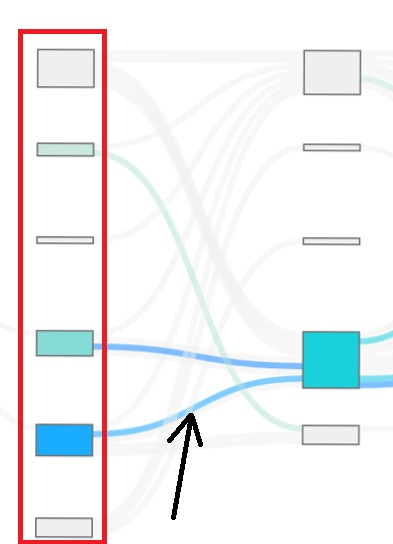
\includegraphics[scale=1]{images/InkedsankeySampleDetail.jpg}
\caption{An enlargement of Figure \ref{fig:sankeysample}, the developer line indicated by black arrow contains data in the time period indicated by red box}
\label{fig:sankeysampledetail}
\end{figure}

The leftmost column shows the raw information about a selected developer, as illustrated in Figure \ref{fig:leftmost}. The large text box contains all paths of the files the selected developer touched in the particular time frame. After selecting a developer, the developer's Github username will be populated after ``Currently selected developer:", the user can then click on the text to jump to that developer's Github profile page. To further assist the user in selecting and finding a developer, if the user hover a particular line, the developer's Github username will be populated above the ``Currently selected developer:" line (we can see the last ``hovered" developer in Figure \ref{fig:leftmost} has the username ``oritwas"). The user can also click on the line to go to that developer's Github profile page.

\begin{figure}[h!]
\centering
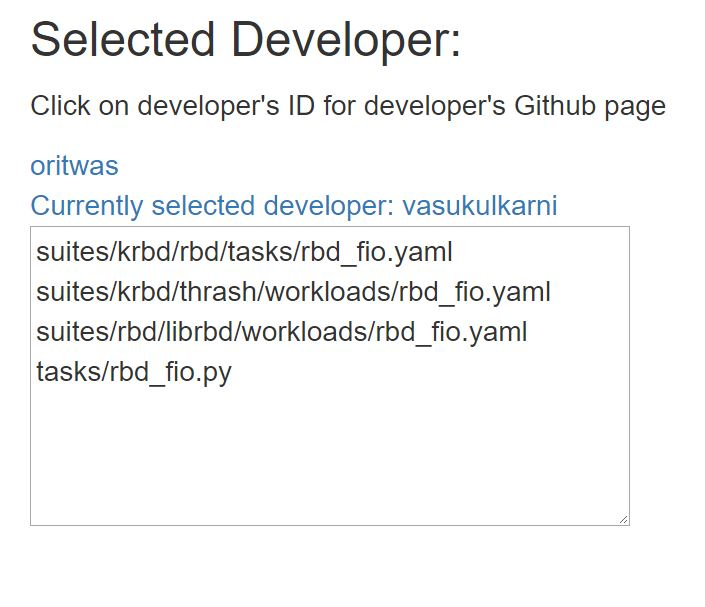
\includegraphics[scale=0.6]{images/leftmost.JPG}
\caption{The leftmost column of the bottom part of the interface showing details of selected developer}
\label{fig:leftmost}
\end{figure}

The center column displays the selected developer's feature focus, as illustrated in Figure \ref{fig:centercol}. The information is compiled on-the-fly from the raw file path data in the leftmost column. The feature focus is presented as a tree where the first node is always named ``root" which represent the entire project. Each node is a potential feature with a percentage number indicating how much does a selected developer work on the feature. The percentage is computed out of ``all files touched." For example, in Figure \ref{fig:centercol}, of all the files this selected developer touched, 75\% of them is under the feature ``suites." Also, out of all files touched, 50\% of them is under the feature ``suites/krbd"

\begin{figure}[h!]
\centering
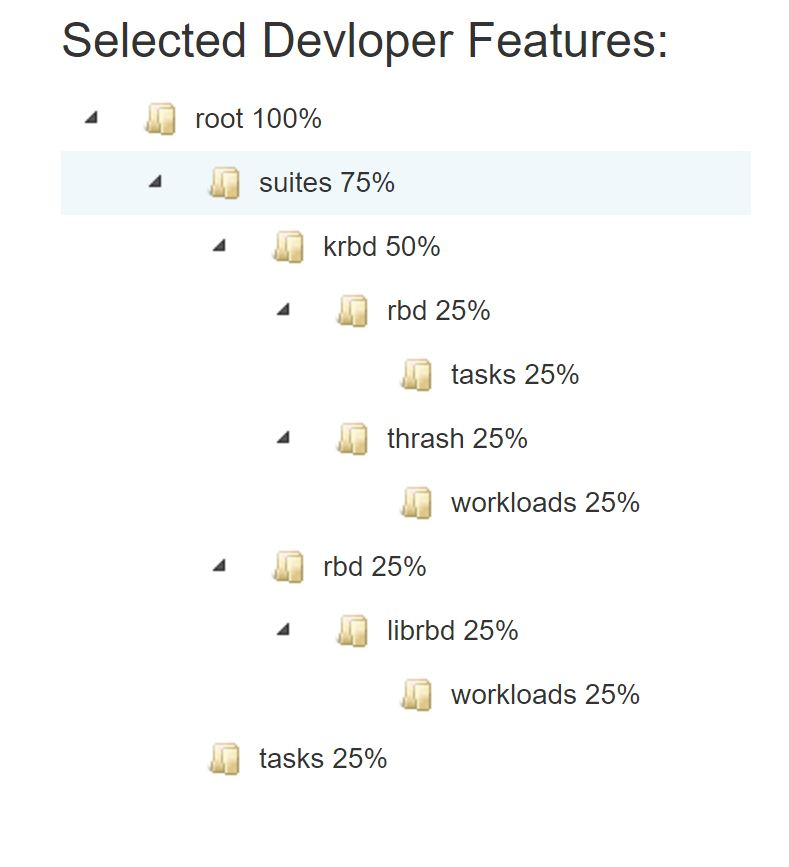
\includegraphics[scale=0.6]{images/center.JPG}
\caption{The center column of the bottom part of the interface showing selected developer's feature focus}
\label{fig:centercol}
\end{figure}

The rightmost column displays a similar feature tree as the center column for a selected cluster, as illustrated in Figure \ref{fig:rightmost}. The annotation for nodes has the same meanings as the center column as discussed above. For example, in Figure \ref{fig:rightmost}, of all the files touched by all the developers in the selected cluster, 10\% of them is under feature ``src/os."\\
In the above 2 columns with feature tree, DECO-X automatically drop the node with the percentage number less than 5\% to prevent clutter. 

\begin{figure}[h!]
\centering
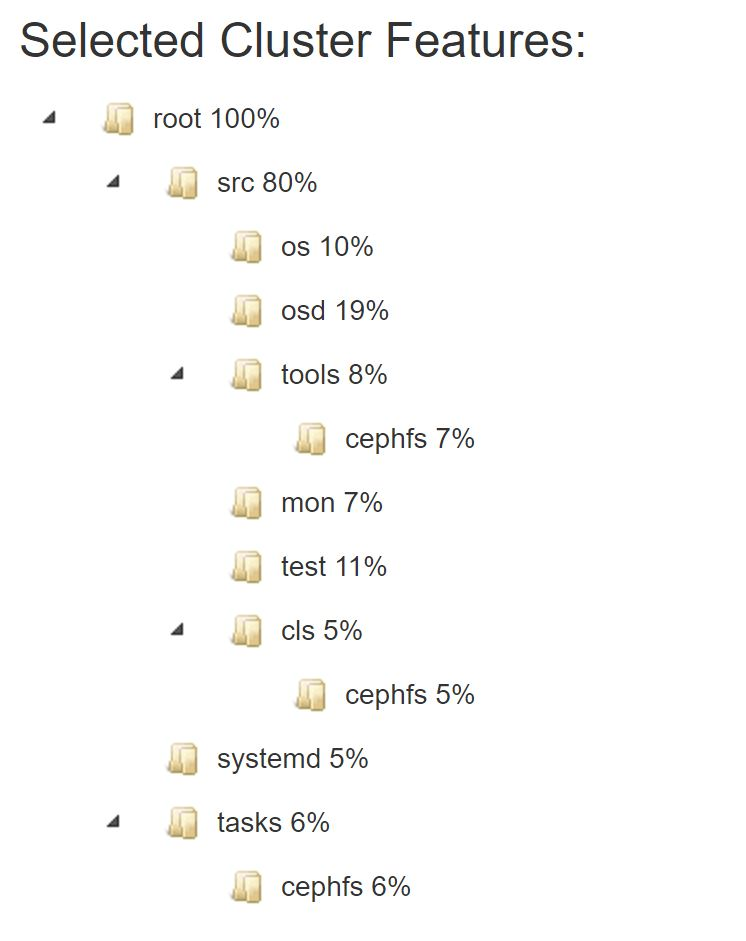
\includegraphics[scale=0.6]{images/rightmost.JPG}
\caption{The rightmost column of the bottom part of the interface showing selected cluster's feature focus}
\label{fig:rightmost}
\end{figure}

Aside from the components mentioned above, DECO-X will display other supportive component such as sliders or modal forms to ask the user for input when needed.
\section{Use Cases}
To demonstrate the effectiveness of DECO-X, we came up with 4 sample use cases that utilize DECO-X to investigate the collaboration between developers in OSS projects. As mentioned before, we will use the project CEPH as a demonstration and we will partition each Sankey diagram to contain only 30 graphs. To minimize for the left censorship effect mentioned above, the demonstration in this section will use graph 390-420 which corresponds roughly to data from November 2015 to June 2016.
\subsection{Use Case 1: Searching For A Developer}
Searching for a developer is probably the one of the most basic analysis on a particular OSS project. Under this case, the user already know the username of a particular developer. Some example uses that might fall under this use case could be:
\begin{itemize}
    \item The user wish to search for a particular developer to investigate his or her work focus over this time period.
    \item The user wish to see if 2 developers frequently worked together.
    \item The user wish to test if a certain set of developers focus on the same feature or not.
\end{itemize}
In this case, the user would choose ``Search For A Developer" under Explore Project Developers. A modal would prompt the user to enter the developer's username and select a color to represent the developer. After clicking ``Search!," the lines represent the developer would be highlighted by the color the user selected. This feature is not destructive meaning the user can repeat this process many times to highlight several developers with different colors, Figure \ref{fig:usecase1} demonstrates such ability. In Figure \ref{fig:usecase1}, the user searched for 2 developers whose usernames are: trociny (red) and tchaikov (blue). With these 2 users highlighted, the user can further investigate their collaboration. For example, we can see from the Figure \ref{fig:usecase1} that these 2 users appear in the same clusters at 2 different time frames (the third and the fifth from the left). The user can then further investigate those clusters by clicking on them. The user can also click on each developer's highlighted line to investigate his or her work focus over time. This might help the investigation of ``focus shifting" as mentioned in the discussion of previous work by Xuan et al.\citep{xuan2014focus}.
\begin{figure}[h!]
\centering
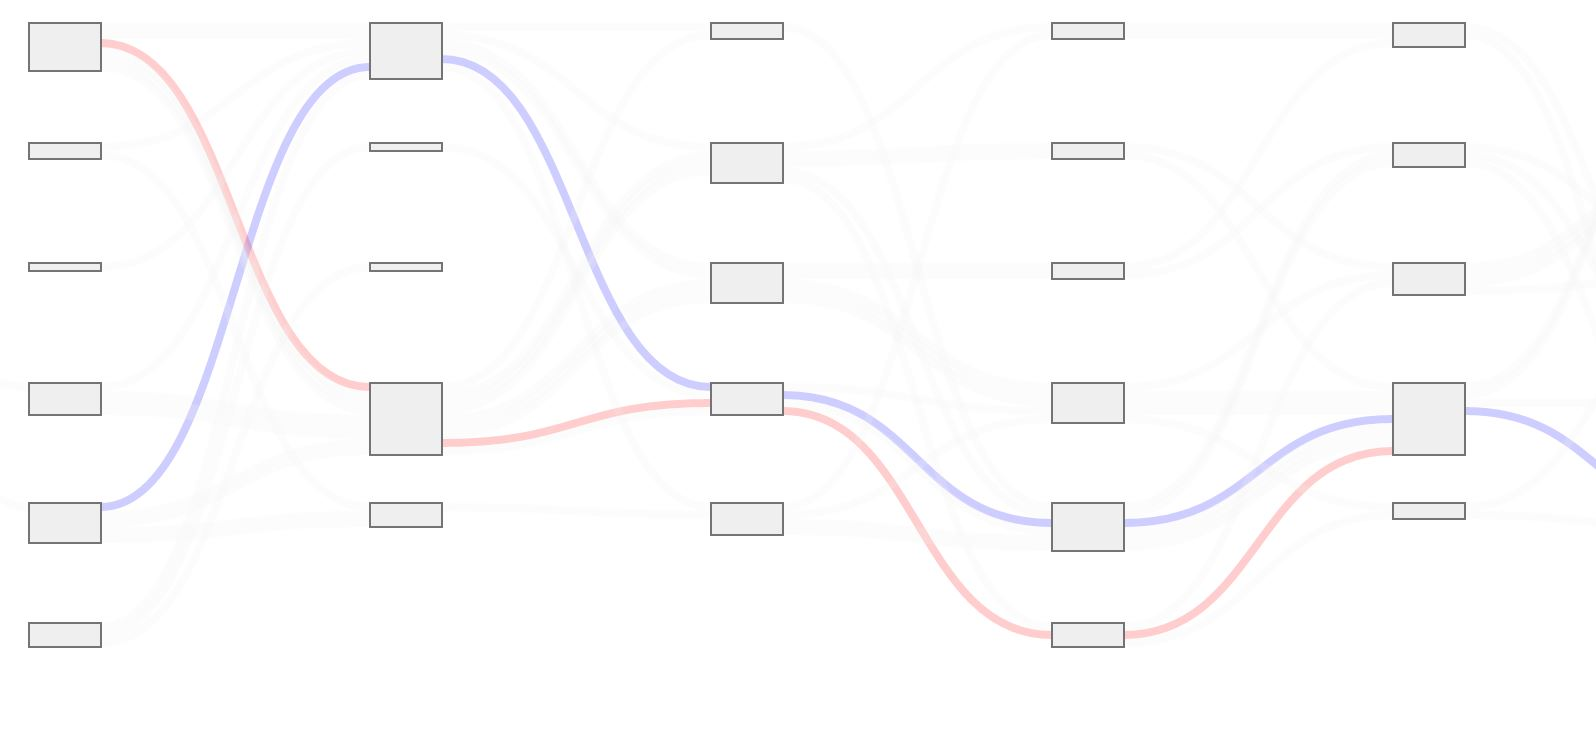
\includegraphics[scale=0.6]{images/usecase1.JPG}
\caption{An example of Use Case 1 with 2 developer highlighted with different colors}
\label{fig:usecase1}
\end{figure}

\subsection{Use Case 2: Search For A Feature}
Similar to searching for developers, the user might want to investigate who is working on a particular feature. Some example uses that might fall under this use case could be:
\begin{itemize}
    \item The user wish to discover the principle developer of a particular feature.
    \item The user wish to discover which clusters of developers worked on a feature.
    \item The user wish to investigate if 2 features are highly related. I.e. when a developer works on feature A, he or she works on feature B.
\end{itemize}
In this use case, the user already know the feature he or she wishes to investigate, say ``src/os." The user would then select ``Search For Feature" under Explore Project Features. After entering the feature and selecting a color (blue in our example), the tool would produce a graph similar to that in Figure \ref{fig:usecase2}. Several things to note when searching for a feature.\\
First, both the clusters and developers are highlighted. The clusters and developers who worked on the feature ``src/os" all will display a shade of blue to allow further investigation.\\
Second, the color for each developer or cluster is interpolated from its current color to the targeted color, the more blue it is, the more the developer or cluster work on the feature. All colors initially are grey. Because of the interpolation algorithm used, some color might not resemble blue as we can observe some purple lines on the right side of Figure \ref{fig:usecase2}. From the graph, we can observed that in each time frame, there's at least one cluster which displayed a deep shade of blue, this suggests that feature ``src/os" could be of high interest for the developers.\\
\begin{figure}[h!]
\centering
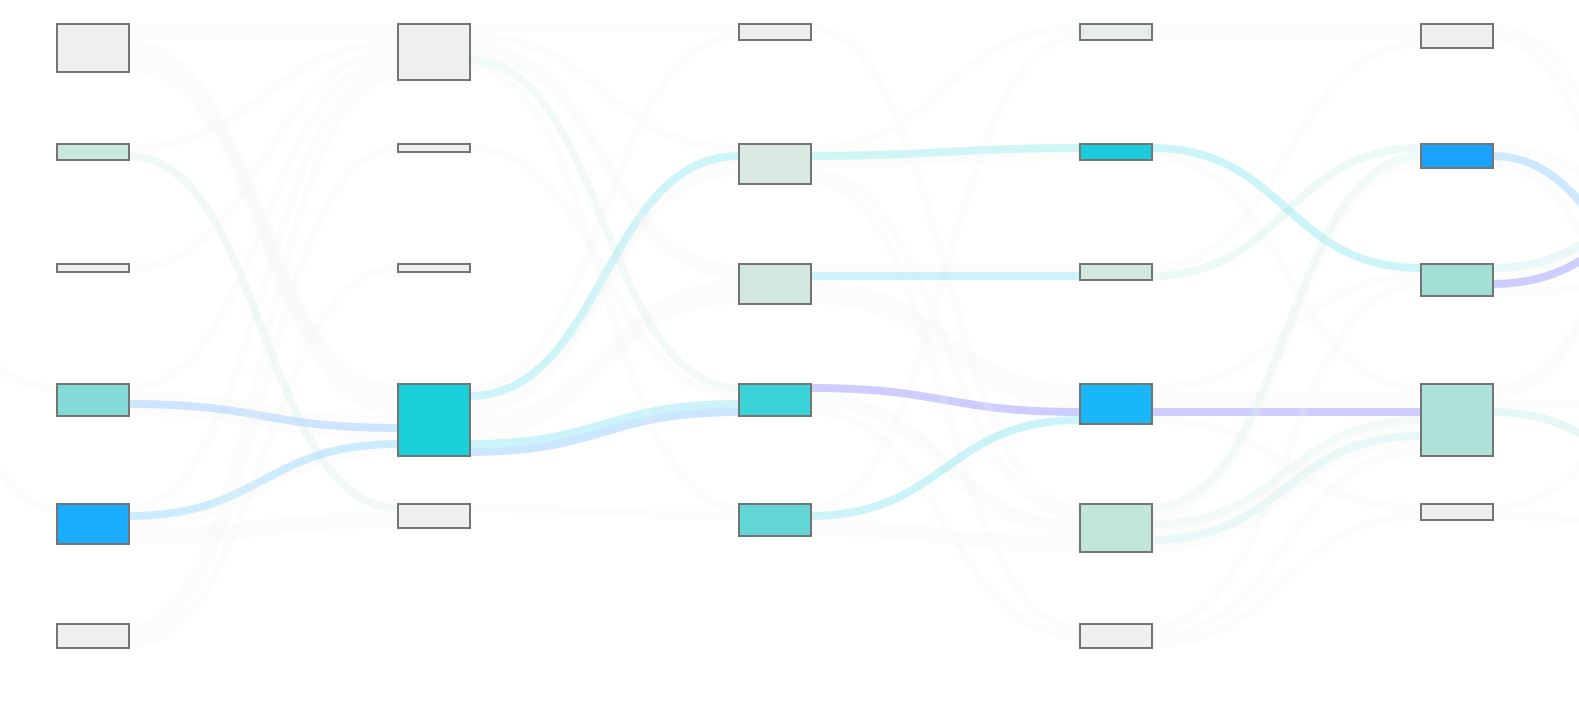
\includegraphics[scale=0.6]{images/usecase2.JPG}
\caption{An example of Use Case 2 with feature ``src/os" highlighted, a developer/cluster who focuses more on ``src/os" displays a darker shad of blue}
\label{fig:usecase2}
\end{figure}
Third, this feature is also non-destructive, the user can search for multiple features and the color will be blended between them. For example, user can search for feature ``src/os" with color blue and another feature ``src/mon" with red by clicking the main menu option 2 times. Then if a color appears to be magenta (the blend between blue and red), then the developer or cluster worked on ``src/mon" and ``src/os" about equally.\\ 
Because of the use of color blending, this function can be used to identify if a developer is multitasking excessively by searching for multiple features with different colors. This can potentially mitigate excessive multitasking and increase productivity, as mentioned in the previous discussion of the work by Vasilescu et al\citep{vasilescu2016sky}.
\subsection{Use Case 3: Search For Developers in Selected Cluster}
When looking at a particular cluster, the user might want to investigate the collaboration of developers in the cluster. Some uses under this use case could be:
\begin{itemize}
    \item The user wish to discover where all the developers in the cluster are coming from and going to. 
    \item The user wish to investigate if a particular cluster of developers stays together all the time.
    \item The user wish to see what the majority of developers in the cluster was working on before (or would be working on afterwards).
\end{itemize}
In this use case, the user has already identified a particular cluster with our tool and selected the cluster by double clicking on the box. The user then can highlight all developers in this cluster with a specified color to investigate the ``flow" of developers in and out of this cluster and track each individual developers, as shown in Figure \ref{fig:usecase3}.
\begin{figure}[h!]
\centering
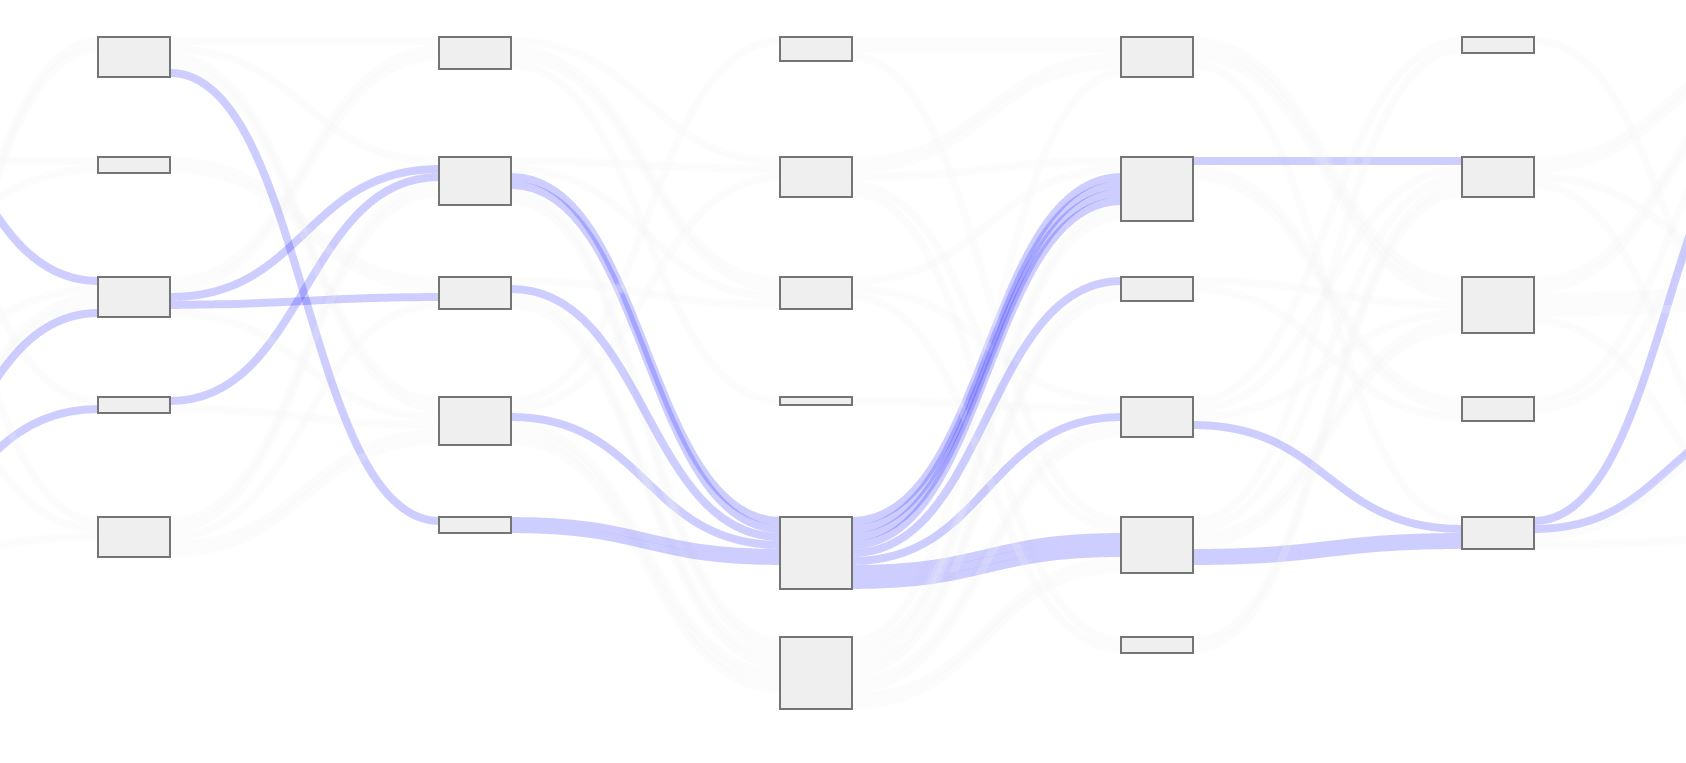
\includegraphics[scale=0.5]{images/usecase3.JPG}
\caption{An example of use case 3 with all developers from a single cluster highlighted}
\label{fig:usecase3}
\end{figure}
Similar to previous use cases, this use case is also non-destructive. The user can select multiple clusters and highlight developers in them by using this function multiple times. However, a developer would only be highlighted in the latest color if he or she exists in multiple clusters.
\subsection{Use Case 4: Search Principle Developers of A Feature}
As suggested by Xuan et al.\citep{xuan2014focus}, developers in OSS projects tend to focus on specific features at a time and that focus shifts over time. As such, the user might want to find out who focuses on a particular feature in the current time frame. Some other uses that fall under this case might be:
\begin{itemize}
    \item The user wish to investigate if a particular feature is being worked on in the specific time frame.
    \item The user wish to see if there are developer who focus more than, say, 50\%, on a particular feature.
\end{itemize}
In this case, the user already identified the feature he or she wishes to investigate. Then, the user would click on ``Search Principle Developers of A Feature" under Explore Project Features. After providing the feature name and color, the Sankey diagram would look similar to Figure \ref{fig:usecase4}.
\begin{figure}[h!]
\centering
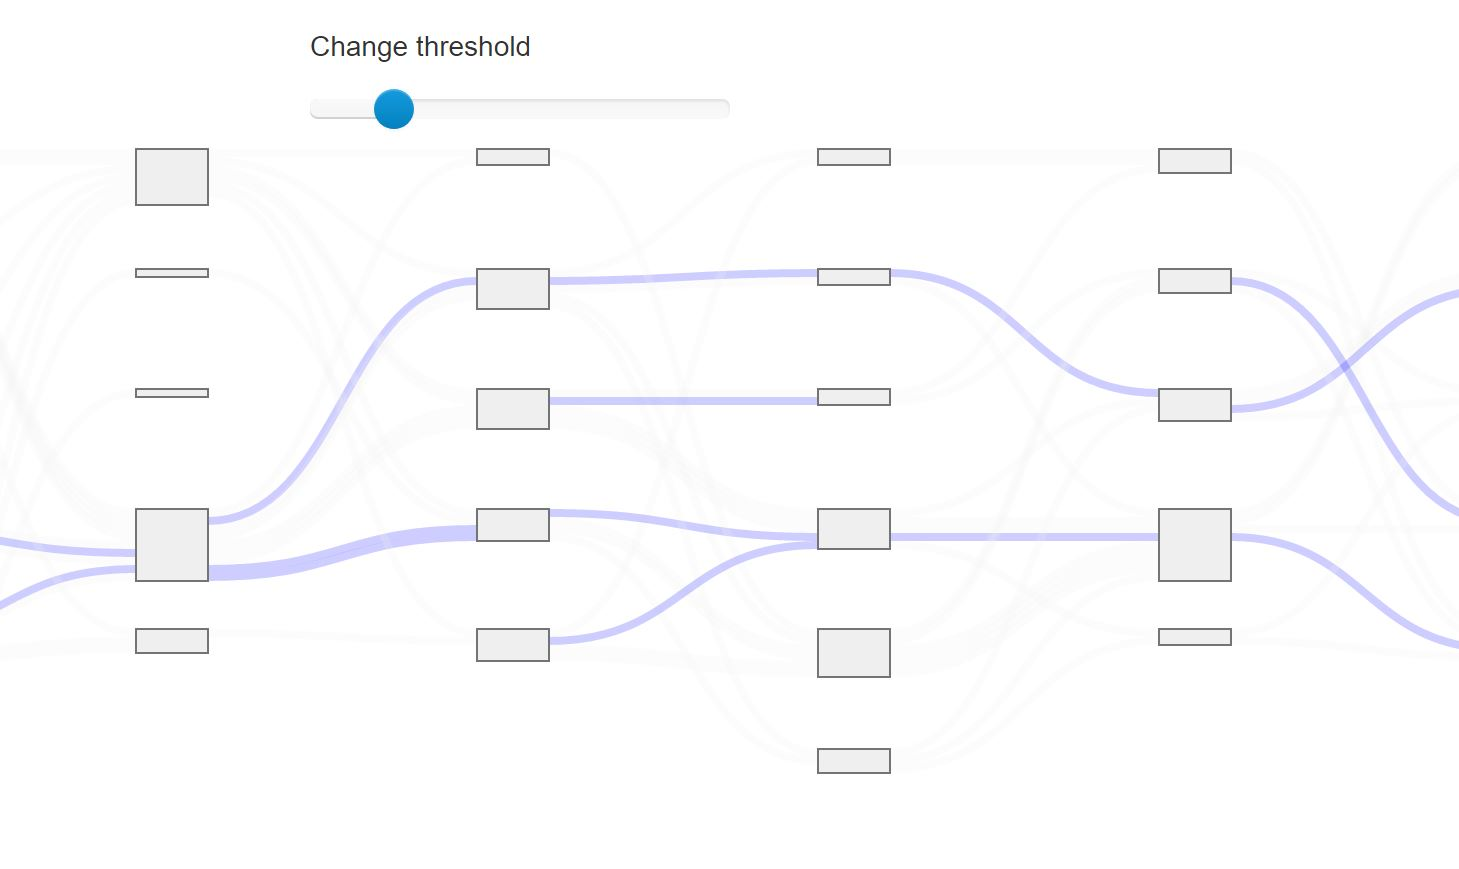
\includegraphics[scale=0.6]{images/usecase4.JPG}
\caption{An example of use case 4 with developer who focuses more than 20\% on ``src/os" highlighted}
\label{fig:usecase4}
\end{figure}
In Figure \ref{fig:usecase4}, the feature being investigated is ``src/os" and we can see several developers are being highlighted. The developers being highlighted in this figure are all the developers whose commit file data contains more than 20\% that are under ``src/os," several things to note here.
First, an additional slider ``Change threshold" shows up above, the user can then use the slider to adjust the threshold that determine whether a developer should be highlighted. After each adjustment, the graph would be updated immediately. For example, if we adjust the threshold to 50\%, meaning only highlight developer whose commit files contains more than 50\% that are in ``src/os," Figure \ref{fig:usecase4-2} would show up.
\begin{figure}[h!]
\centering
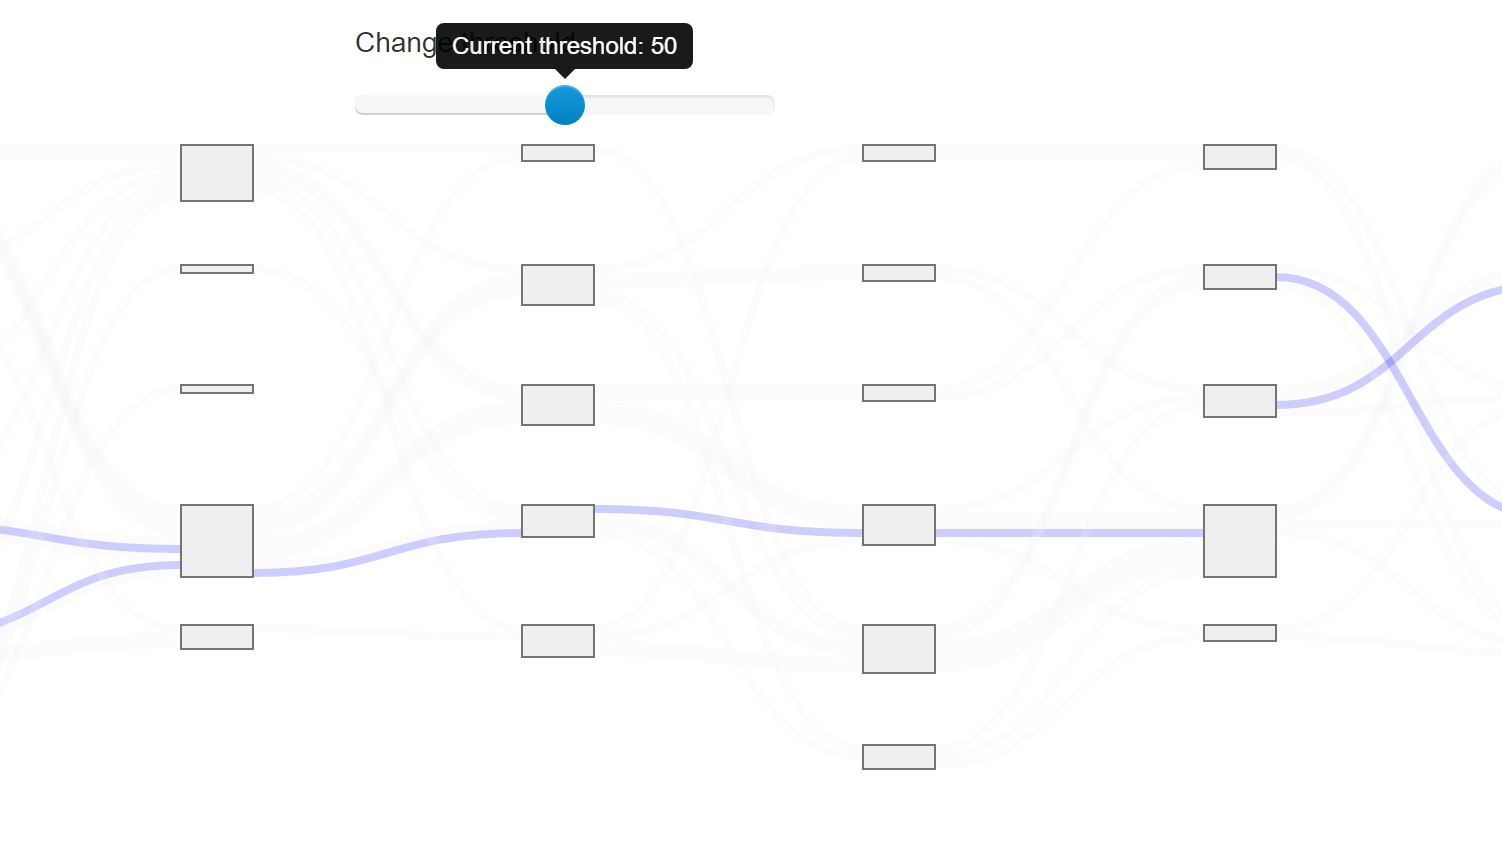
\includegraphics[scale=0.6]{images/usecase4-2.JPG}
\caption{The same example as Figure \ref{fig:usecase4} with threshold changed to 50\%}
\label{fig:usecase4-2}
\end{figure}
We can see some developers that are highlighted in Figure \ref{fig:usecase4} is not highlighted anymore as their commit file data contains more than 20\% of ``src/os" but no more than 50\%.\\
Second, because of the need to update graph in real-time, this feature is destructive. Meaning if there are previously highlighted developers, using this feature would erase them.\\
During our analysis of CEPH, we find that in the inspected time frame, the developers whose works contain more than 65\% in feature ``src/os" includes Github user: XinzeChi, majianpeng, yuyuyu101, shinobu-x and athanatos. Very interestingly, former 4 out of these 5 developers are all based in Asia (with former 3 based in China) according to their Github profile. This could have several implications. For example, with almost all developers working on ``src/os" based in Asia, this could suggest that the majority of the work on ``src/os" is done during normal hours in Asian time so other developers might need to adjust their working schedule to collaborate the ``src/os" team.
\section{Conclusions}
In this project, we proposed a complete pipeline that allows the user to explore any generic Github project. All the user would need is the project's name to start using DECO-X, as shown by our demonstration of the analysis of CEPH. Because of DECO-X's focus on repository history, interesting questions such as ``what are the developers' focuses 3 months ago" can be answered with ease. As such, this can be potentially very helpful for many people involved in OSS projects. Going back to our fictional project, ``COOSOFT," Vlad can use DECO-X to find out what was the popular feature in the past couple weeks by utilizing Use Case 2. Prem can discover who worked or is working on operating system related features by utilizing Use Case 4. And, Cindy can discover the dominant developers by investigating the commit file data with DECO-X's interface easily. Lastly, Casey, the university researcher, can utilize DECO-X to investigate how the focus of each developer shifts over time and the collaborations between developers with little efforts.
\subsection{Limitations And Threats to Validity}
Several limitations are present in DECO-X. First, based on the current design, the gathering of commit file data is very time consuming. Also, because of the fact that commits from long ago could have been deleted, the data gathered might exhibit a left censorship effect as mentioned above. Similarly, an OSS project with very few commits might also render this tool ineffective because of the sparsity of data. These could be mitigated by investigating a more current, active OSS project with shorter history. Second, the construction of the graph are based on user defined criteria. This might be quite subjective and does not capture the collaboration between developers. Similarly, for the clustering and embedding, several user adjustable parameters are present and they all could affect the visualization drastically thus hinder the investigation. During our experiments, we found that the embedding and clustering algorithm affects the results the most. For example, with an ineffective clustering algorithm, the developers might not be clustered properly thus investigating the ``flow of developers" might produce useless data. Also, choosing between KM clustering and HC would also greatly impact the result. Moreover, it is especially hard to come up with the ``correct" clustering criteria that properly cluster developers based on their feature focus. The 2 approaches we suggested both suffers from the fact that an previous assumption about how the developer collaborated must be made in order to make the clustering algorithms work. Such as the one in our analysis, where we assumed that ``number of cluster in each time frame graph is in sub-linear relation to number of developers."
\subsection{Future Works}
In the future, there's several places of this tool that can be improved. First and utmost, a creative clustering and embedding technique could be implemented so that there will be no need for a previous assumption of the clusters. With this, DECO-X can fully automate the discovery of clusters without any user intervention.\\
Second, more use cases can be developed. We have shown 4 use cases that demonstrate the flexibility of the UI which can potentially lead to more functions. For example, utilizing the ``slider control" used in use case 4, we could develop, say, a function that automatically discovers the dominant developers by setting an adjustable threshold for ``number of files touched" when searching for developers. Another example, we might be able to incorporate the ``color blending" used in use case 2 to use it to highlight developers who frequently worked together in the following way: set a color for each developer and the more 2 developer works together, the more blended their color is.\\
Third, the data gathering module can be expanded to include a ``deep analysis" of the raw git data which can compensate for the left censorship effect of commit file data. Instead of just using commits that exists for file data, the tool could be expanded to analyze the raw git history from the git files which could include file data in earlier deleted commits.\\
Fourth, relating the limitation that an assumption must be made about the collaboration as mentioned above, more works can be put into validating such an assumption by statistical analysis. Since our tool allows the easy investigation of collaboration and developer activities, it could be possible to use the visualization interface in reverse to gauge how good the clustering or embedding algorithm is.
\bibliographystyle{plain}
\bibliography{references}
\end{document}
